	\subsection{Second-Order System}

We collect the equations of the shunt voltages, e.g. Eq.  (\ref{eq:rl-c_shunt_ode_0}, \ref{eq:rl-c_shunt_ode_n}), and we arrange them as a system of second order equations
\begin{equation}
	M~ \ddot{z}(t) + D~ \dot{z}(t) + S~ z(t) = G ~ \mu(t)
	\label{eq:rlc_second_order_1}
\end{equation}
with matrices $M = \left[ m_{n,k} \right]$, $D = \left[ d_{n,k} \right]$ and  $S = \left[ s_{n,k} \right]$, and vectors $z$ as in Eq. \eqref{eq:z_voltages_shunt} and  $G = [1, 0, \ldots, 0]^{\top}$. The indices of our matrix elements denote a row $n\in \{1,\ldots,N\}$ and column $k\in \{1,\ldots,N\}$. This index notation refers to the indices in the voltage differential equations, e.g. Eq. (\ref{eq:rl-c_shunt_ode_n}, \ref{eq:rl-c_shunt_ode_0}) etc. The input signal $\mu(t)$ identifies either $u(t)$ for circuit \ref{fig:cascaded_rlc_circuits} (a), $\partial_{t} u(t) = \dot{u}(t)$  for circuit (b) or  $\partial_{t}^2 u(t) = \ddot{u}(t)$ for circuit (c).

The symbols of these matrices, $M$, $D$ and $S$, refer to the mass, damping and stiffness in mechanical systems. Our modeling approach of the second-order systems results in two types of matrices: upper triangular shapes and lower finite difference stencils, see the matrix shapes in Fig. \ref{fig:matrix_shapes}. The upper triangular matrices have a shape as
\begin{equation}
	\mathbf{T}_{a,b} = 
	\begin{pmatrix}
		a_{1} b_{1} & a_{1} b_{2} & \cdots &  a_{1} b_{N-1} & a_{1} b_{N} \\
		0 			& a_{2} b_{2} & \cdots &  a_{2} b_{N-1} & a_{2} b_{N} \\
		\vdots			& \ddots	  & \ddots &  \vdots        & 	\vdots	  \\
		&			  &        & a_{N-1} b_{N-1}& a_{N-1} b_{N} \\
		0			&	\cdots		  &        &	0            & a_{N} b_{N} 
	\end{pmatrix}
	\label{eq:triangular_matrix} 
\end{equation}
where our coefficients $(a_{n}, b_{k})$ with $n,k \in \{1,\ldots,N\}$ stand for the related electrical coefficients and their reciprocals, see Equations (\ref{eq:rl-c_shunt_ode_n}, \ref{eq:rl-c_shunt_ode_0}), (\ref{eq:lc-r_shunt_ode_n}, \ref{eq:lc-r_shunt_ode_0}) and (\ref{eq:rc-l_shunt_ode_n},\ref{eq:rc-l_shunt_ode_0}), and Table \ref{table:triangular_matrix_values}. The finite difference stencil is
\begin{equation}
	\mathbf{F} = 
	\begin{pmatrix}
		1 & 0 & \cdots &  &  0\\
		-1 			& 1 & 0 &   & \vdots  \\
		0 & \ddots	  & \ddots & \ddots  & 	 \\
		\vdots &			  &     -1  & 1 &  0 \\
		0 &	\cdots		  &     0   & -1  & 1 
	\end{pmatrix} 
	\textbf{.}
	\label{eq:finite_diff_stencil} 
\end{equation}
The matrix entries for each circuit type are noted in Table \ref{table:overview_matrix_entries}. The triangular matrix structure corresponds to a spatially discrete integration and the finite difference shape to a differentiation.  We assume, $R_{n}$, $L_{n}$, $C_{n} \in \mathbb{R}_{>0} \setminus \{\infty\}$ and so the resulting triangular matrices are invertible. Hence, we are able to reformulate the second-order system via inverse matrix multiplication as first-order system. 

\begin{margintable}
	\renewcommand{\arraystretch}{1.3}
	\centering
	\caption{{Triangular Matrix Corresponding Values}}
	\begin{tabular}{l l l l}
		\toprule
		Shunt & Matrix & $a_{n}$ & $b_{k}$ \\
		\midrule
		Capacitor & M & $L_{n}$ & $C_{k}$	\\
		& D & $R_{n}$ & $C_{k}$ \\[1.5ex] 
		Resistor & M & $L_{n}$ & $R_{k}^{-1}$ \\ 
		& S & $C_{n}^{-1}$ & $R_{k}^{-1}$ \\[1.5ex] 
		Inductor & D & $R_{n}$ & $L_{k}^{-1}$ \\
		& S & $C_{n}^{-1}$ & $L_{k}^{-1}$ \\ 
		\bottomrule
	\end{tabular}
	\label{table:triangular_matrix_values}	
\end{margintable}

%\begin{table}[b]
%	\renewcommand{\arraystretch}{1.3}
%	\centering
%	\caption{\MakeUppercase{Triangular Matrix Corresponding Values}}
%	\begin{tabular}{l l l l}
%		\toprule
%		Shunt & Matrix & $a_{n}$ & $b_{k}$ \\
%		\midrule
%		Capacitor & M & $L_{n}$ & $C_{k}$	\\
%		& D & $R_{n}$ & $C_{k}$ \\[1.5ex] 
%		Resistor & M & $L_{n}$ & $R_{k}^{-1}$ \\ 
%		& S & $C_{n}^{-1}$ & $R_{k}^{-1}$ \\[1.5ex] 
%		Inductor & D & $R_{n}$ & $L_{k}^{-1}$ \\
%		& S & $C_{n}^{-1}$ & $L_{k}^{-1}$ \\ 
%		\bottomrule
%	\end{tabular}
%	\label{table:triangular_matrix_values}
%\end{table}


\begin{figure}[t!]
	\centering
	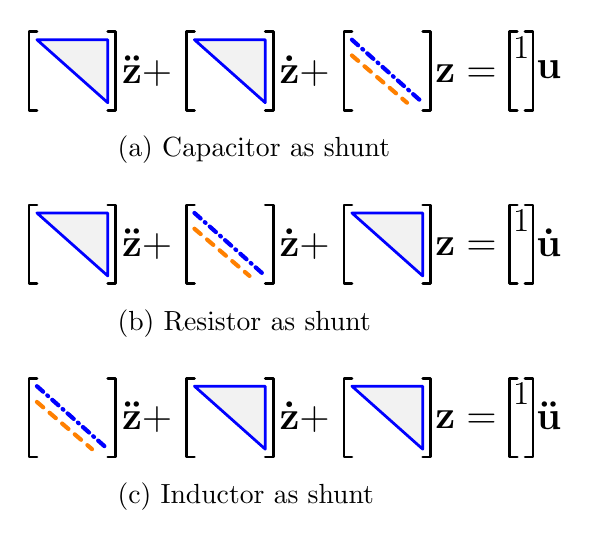
\begin{tikzpicture}[scale=1,line cap=round,line join=round,x=1.0cm,y=1.0cm]	
		\def\dx{2};
		\def\dy{2.2};
		
		\foreach \i in {0, 1, 2}
		{
			\draw[line width=1.0] (0.1+\i*\dx,0+\dy) -- (0+\i*\dx,0+\dy) -- (0+\i*\dx,1+\dy) -- (0.1+\i*\dx,1+\dy);
			\draw[line width=1.0] (1.0+\i*\dx,0+\dy) -- (1.1+\i*\dx,0+\dy) -- (1.1+\i*\dx,1+\dy) -- (1.0+\i*\dx,1+\dy);
		}
		\node at (1.5,0.5+\dy) {\Large $\mathbf{\ddot{z}}+$};
		\node at (1.5+\dx,0.5+\dy) {\Large $\mathbf{\dot{z}}+$};
		\node at (1.55+2*\dx,0.47+\dy) {\Large $\mathbf{z}=$};
		
		\draw[line width=1, color=blue, fill=gray!10] (0.1, 0.9+\dy) -- (1.0, 0.9+\dy) -- (1.0, 0.1+\dy) -- cycle;
		\draw[line width=1, color=blue, fill=gray!10] (0.1+\dx, 0.9+\dy) -- (1.0+\dx, 0.9+\dy) -- (1.0+\dx, 0.1+\dy) -- cycle;
		\draw[dash dot,line width=1.5, color=blue] (0.1+2*\dx,0.9+\dy) -- (1.+2*\dx,0.1+\dy);
		\draw[dashed,line width=1.5, color=orange] (0.1+2*\dx,0.7+\dy) -- (0.8+2*\dx,0.1+\dy);
		\draw[line width=1.0] (0.2+3*\dx,0+\dy) -- (0.1+3*\dx,0+\dy) -- (0.1+3*\dx,1+\dy) -- (0.2+3*\dx,1+\dy);
		\draw[line width=1.0] (0.3+3*\dx,0+\dy) -- (0.4+3*\dx,0+\dy) -- (0.4+3*\dx,1+\dy) -- (0.3+3*\dx,1+\dy);
		\node at (0.25+3*\dx,0.8+\dy) {\large $1$};
		\node at (0.6+3*\dx,0.52+\dy) {\Large $\mathbf{u}$};
		
		\node[right] at (1.0, -0.5+\dy) {(a) Capacitor as shunt};
		
		
		\foreach \i in {0, 1, 2}
		{
			\draw[line width=1.0] (0.1+\i*\dx,0) -- (0+\i*\dx,0) -- (0+\i*\dx,1) -- (0.1+\i*\dx,1);
			\draw[line width=1.0] (1.0+\i*\dx,0) -- (1.1+\i*\dx,0) -- (1.1+\i*\dx,1) -- (1.0+\i*\dx,1);
		}
		\node at (1.5,0.5) {\Large $\mathbf{\ddot{z}}+$};
		\node at (1.5+\dx,0.5) {\Large $\mathbf{\dot{z}}+$};
		\node at (1.55+2*\dx,0.47) {\Large $\mathbf{z}=$};
		\draw[line width=1, color=blue, fill=gray!10] (0.1, 0.9) -- (1.0, 0.9) -- (1.0, 0.1) -- cycle;
		\draw[line width=1, color=blue, fill=gray!10] (0.1+2*\dx, 0.9) -- (1.0+2*\dx, 0.9) -- (1.+2*\dx, 0.1) -- cycle;
		\draw[dash dot,line width=1.5, color=blue] (0.1+\dx,0.9) -- (1.+\dx,0.1);
		\draw[dashed,line width=1.5, color=orange] (0.1+\dx,0.7) -- (0.8+\dx,0.1);
		\draw[line width=1.0] (0.2+3*\dx,0) -- (0.1+3*\dx,0) -- (0.1+3*\dx,1) -- (0.2+3*\dx,1);
		\draw[line width=1.0] (0.3+3*\dx,0) -- (0.4+3*\dx,0) -- (0.4+3*\dx,1) -- (0.3+3*\dx,1);
		\node at (0.25+3*\dx,0.8) {\large $1$};
		\node at (0.6+3*\dx,0.52) {\Large $\mathbf{\dot{u}}$};
		
		\node[right] at (1.0, -0.5) {(b) Resistor as shunt};
		
		
		\def\dy{-2.2};
		\foreach \i in {0, 1, 2}
		{
			\draw[line width=1.0] (0.1+\i*\dx,0+\dy) -- (0+\i*\dx,0+\dy) -- (0+\i*\dx,1+\dy) -- (0.1+\i*\dx,1+\dy);
			\draw[line width=1.0] (1.0+\i*\dx,0+\dy) -- (1.1+\i*\dx,0+\dy) -- (1.1+\i*\dx,1+\dy) -- (1.0+\i*\dx,1+\dy);
		}
		\node at (1.5,0.5+\dy) {\Large $\mathbf{\ddot{z}}+$};
		\node at (1.5+\dx,0.5+\dy) {\Large $\mathbf{\dot{z}}+$};
		\node at (1.55+2*\dx,0.47+\dy) {\Large $\mathbf{z}=$};
		\draw[dash dot,line width=1.5, color=blue] (0.1,0.9+\dy) -- (1.,0.1+\dy);
		\draw[dashed,line width=1.5, color=orange] (0.1,0.7+\dy) -- (0.8,0.1+\dy);
		\draw[line width=1, color=blue, fill=gray!10] (0.1+\dx, 0.9+\dy) -- (1.0+\dx, 0.9+\dy) -- (1.0+\dx, 0.1+\dy) -- cycle;
		\draw[line width=1, color=blue, fill=gray!10] (0.1+2*\dx, 0.9+\dy) -- (1.0+2*\dx, 0.9+\dy) -- (1.+2*\dx, 0.1+\dy) -- cycle;
		\draw[line width=1.0] (0.2+3*\dx,0+\dy) -- (0.1+3*\dx,0+\dy) -- (0.1+3*\dx,1+\dy) -- (0.2+3*\dx,1+\dy);
		\draw[line width=1.0] (0.3+3*\dx,0+\dy) -- (0.4+3*\dx,0+\dy) -- (0.4+3*\dx,1+\dy) -- (0.3+3*\dx,1+\dy);
		\node at (0.25+3*\dx,0.8+\dy) {\large $1$};
		\node at (0.6+3*\dx,0.52+\dy) {\Large $\mathbf{\ddot{u}}$};
		
		\node[right] at (1.0, -0.5+\dy) {(c) Inductor as shunt};
		
	\end{tikzpicture}
	\caption{Matrix shapes of alternative RLC circuit ladders.}
	\label{fig:matrix_shapes}
\end{figure}


